% Root entry for the supplied ZIP template (ACM sigconf review).
\pdfminorversion=7
\pdfmapfile{+symbols.map}
\pdfmapfile{+cm.map}
\pdfmapfile{+cmextra.map}
\documentclass[sigconf,review,nonacm]{acmart}
\setcopyright{none}
\settopmatter{printacmref=false,printfolios=true}
\usepackage{booktabs,multirow,array,makecell}
\let\Bbbk\relax
\usepackage{amsmath,amssymb}
\usepackage{graphicx,subfigure}
\usepackage{needspace,placeins,pifont,xspace,xstring}
\usepackage[ruled,vlined,linesnumbered]{algorithm2e}
\usepackage{cleveref}
\setlength{\subfigcapskip}{1pt}
\setcounter{dbltopnumber}{3}
\renewcommand{\topfraction}{0.92}
\renewcommand{\dbltopfraction}{0.95}
\renewcommand{\textfraction}{0.07}
\renewcommand{\floatpagefraction}{0.8}
\renewcommand{\dblfloatpagefraction}{0.60}
\newcommand{\LIMIT}{\textsf{LIMIT}\xspace}
\newcommand{\qpm}[2]{#1\,{\scriptsize$\pm$#2}}
\newcommand{\stitle}[1]{\vspace{1ex}\noindent\textbf{#1}}
\newcommand{\cmark}{\ding{51}}
% Default path: evidence off, no input shuffle.
% The objective is estimated merge input tokens; no unverified cost formula is used.
% Full materializes each pass. LIMIT pulls the same groups and stops at K.
% h=1 is LT(h), not a second family.
\DontPrintSemicolon
\newcommand{\Rank}{\mbox{\textsc{ListwiseRank}}}
\newcommand{\Replay}{\mbox{\textsc{Replay}}}
\newcommand{\Refresh}{\mbox{\textsc{Refresh}}}
\newcommand{\MergeGroup}{\mbox{\textsc{MergeGroup}}}
\newcommand{\Expect}{\ensuremath{\mathrm{Expect}}}
\SetKwProg{Fn}{procedure}{:}{}
\SetAlgoNlRelativeSize{-1}
\SetAlFnt{\footnotesize}
\SetAlCapFnt{\footnotesize}
\SetAlgoSkip{}
\SetAlgoInsideSkip{}
\makeatletter
% algorithm2e rejects [H] in two-column mode. Measure the column box, then
% move the whole algorithm to the next column when it does not fit.
% \Needspace comes from the integration preamble; the fallback keeps the
% specialist preview compiling if that package was not loaded.
\providecommand{\Needspace}[1]{}
\newsavebox{\algcolbox}
\newcommand{\algcolstart}{%
  \par
  \begin{lrbox}{\algcolbox}%
  \begin{minipage}[t]{\columnwidth}%
  \@twocolumnfalse
}
\newcommand{\algcolend}{%
  \end{minipage}%
  \end{lrbox}%
  % minipage[t] stores the body as depth. Raise it so the page builder
  % sees the whole algorithm above the baseline and cannot hang off the page.
  \setbox\algcolbox=\hbox{\raise\dp\algcolbox\box\algcolbox}%
  \typeout{ALGBOX ht=\the\ht\algcolbox dp=\the\dp\algcolbox}%
  \Needspace{\dimexpr\ht\algcolbox+\dp\algcolbox+6pt\relax}%
  \noindent\usebox{\algcolbox}\par\smallskip
}
\makeatother


% Keep the figure with its caption in this results scaffold. Once prose is
% available, the normal floats can be reinstated by omitting these wrappers.
\makeatletter
\newsavebox{\manuscriptfigure}
\newcommand{\placeexperimentfigures}{%
  \renewenvironment{figure}[1][]{%
    \par\setbox\manuscriptfigure=\vbox\bgroup
      \hsize=\columnwidth
      \linewidth=\columnwidth
      \captionsetup{type=figure}%
      \centering
  }{%
    \egroup
    \Needspace{\dimexpr\ht\manuscriptfigure+\dp\manuscriptfigure+6pt\relax}%
    \noindent\usebox\manuscriptfigure\par\smallskip
  }%
}
\makeatother

\begin{document}
\title{Cost-effective Multi-way Merge Semantic ORDER BY}
\author{Anonymous Author(s)}
\renewcommand{\shortauthors}{Anonymous}
\begin{abstract}
A listwise language model can rank a batch of rows by a natural-language criterion. When a semantic \textsf{ORDER BY} query exceeds the batch capacity, the operator must merge the resulting runs without spending a model call on every output row. We use external $k$-way merge with two group mergers. Sliding-window merge ranks the heads and nearby rows of several runs, then carries the unreturned rows into the next window. Segmented loser-tree merge keeps the losers at internal nodes and refreshes only one path at a time. Full ranking materializes each merge layer; \LIMIT~$K$ pulls rows from its input groups as needed. The planner estimates the number of calls and the number of rows submitted across those calls, then selects the feasible plan with the lowest estimated input token cost.
\end{abstract}
\maketitle
{\emergencystretch=1em\relax\section{Introduction}

Large Language Models (LLMs) are increasingly used to process unstructured data due to their strong capabilities in semantic understanding and reasoning.
Modern data platforms have begun to develop LLM-powered semantic operators or User-Defined Functions (UDFs), including commercial systems such as Google BigQuery~\cite{google2026bigqueryai}, Snowflake Cortex AI~\cite{snowflake2026cortexai}, and Alibaba PolarDB for AI~\cite{alibaba2026polardbai}, as well as prototype systems for semantic query processing~\cite{DBLP:journals/pvldb/PatelJPGAGZ25}.
This integration poses new problems for physical optimization in database systems. 
Unlike classical relational operators, LLM-powered operators invoke a model on individual records or batches. Each request repeats the ranking instruction and includes the text of every row it compares. Reducing the request count can therefore save tokens, but a plan with fewer requests can still cost more if it resubmits more text.

Among semantic operators, semantic \textsf{ORDER BY} supports queries whose ordering criterion is expressed in natural language.
For example, ordering reviews by their helpfulness for a purchase decision, passages by the strength of their evidential support, or retrieved documents by their relevance to a user question. 
Such functionality is central to document reranking in retrieval-augmented generation (RAG)~\cite{DBLP:conf/nips/YuP0WYZSC24} and semantic search. As semantic \textsf{ORDER BY} requires an LLM to infer a global ordering over input items, when the input exceeds the effective context window of the LLM, no single invocation can inspect all items and produce a global ordering. 
A natural solution is divide-and-conquer sorting: inferring the local order of item subsets that fit in a context window, and combining local orders into a global order. 
This makes processing Semantic \textsf{ORDER BY} substantially more difficult than processing record-independent operators such as semantic filtering. 


Existing LLM ranking methods use pointwise scores, pairwise comparisons, or listwise permutations. Pointwise methods score items independently, which makes scores from different prompts difficult to calibrate~\cite{DBLP:conf/emnlp/DrozdovZD0RWAIM23,DBLP:conf/emnlp/SachanLJAYPZ22}. Pairwise methods compare two items at a time and combine these judgments into a ranking~\cite{DBLP:conf/acl/LuoCH024,DBLP:conf/naacl/QinJHZWYSLLMWB24}. We focus on listwise ranking, which orders an entire batch in one call~\cite{DBLP:conf/emnlp/0001YMWRCYR23,DBLP:journals/corr/abs-2603-17223,DBLP:journals/corr/abs-2509-00303}. The physical operator decides how to turn these local permutations into a full order or an ordered prefix.

Existing operators organize these calls in different ways. ListK studies tournament selection and multi-pivot partitioning~\cite{DBLP:journals/corr/abs-2603-17223}. TBS retains prior judgments in a preference graph and skips batches whose pairwise orders are already implied~\cite{akinola2026tbs}. Two-way external merge instead generates sorted runs and uses their ordered heads to assemble the result~\cite{DBLP:journals/corr/abs-2509-00303}. A merge call can contain rows whose relative order is already known. A wider fan-in reduces the number of passes, but it also changes how many rows can enter each call and how often they return to the prompt. The number of known pairs in a batch does not tell us which plan spends fewer input tokens.

The key observation is that a run needs to supply only enough rows to determine what can be emitted next. A sliding window retains rows that cannot yet be emitted and replenishes each active run. A segmented loser tree retains the losing segments and reranks only one path on a refill. These two choices of merge group expose different trade-offs between the number of calls and the number of row appearances. Output demand changes the trade-off again: Full ranking drains every group, while a small \LIMIT~$K$ can stop after consuming uneven prefixes from different children, even though both modes generate all initial runs.

Figure~\ref{fig:framework} illustrates why one plan need not serve both queries. Given the same initial runs, the planner can choose different mergers, fan-ins, and segment lengths for Full and \LIMIT~$K$. It estimates the work of each feasible plan under the requested output demand and prices it using the query's prompt profile.

\textbf{Contributions.}
\begin{itemize}
  \item \textbf{Multi-way listwise merge.} We develop a sliding-window merger with safe-prefix emission and a segmented loser tree with pointer-guided refresh. The same groups support materialized full ranking and demand-driven ordered prefixes. We establish correctness under a consistent ordering oracle.
  \item \textbf{Demand-aware plan selection.} We estimate the calls and row appearances of each feasible merge plan by replaying its finite execution. A token profile fits the fixed request cost and per-row cost without labeled rankings or model generation. The planner chooses the family, fan-in, and quota or segment length for the requested demand.
  \item \textbf{Evaluation.} We study end-to-end ranking quality, token use, and latency, and isolate plan selection, input scale, prefix caching, and the change from small limits to full ranking.
\end{itemize}
\par}
{\emergencystretch=2em\relax\section{Preliminaries}
\label{sec:prelim}

\stitle{Semantic \textsf{ORDER BY}.}
Let $D=\{x_1,\dots,x_n\}$ be a collection of $n$ items, such as documents, passages, or records with unstructured text fields. 
Let $\phi$ be a natural-language instruction that specifies a desired ordering criterion, e.g., \emph{``order the reviews from most to least helpful for a purchase decision''}. 
A semantic \textsf{ORDER BY} operator returns a permutation $\Pi = [\pi_1, \cdots, \pi_n]$ of $D$ that is consistent with the order criterion induced by $\phi$. We assume the permutation $\Pi$ is in non-decreasing order throughout this paper. 
Unlike conventional \textsf{ORDER BY}, where the ordering key is a deterministic attribute value that can be compared directly by database engine, the semantic \textsf{ORDER BY},  defined through natural-language semantics, may depend on implicit notions such as relevance, helpfulness, specificity, sentiment, or evidential support, and therefore cannot be evaluated by a traditional comparator. We use a large language model (LLM) as an ordering oracle for this semantic relation. 

This LLM-based formulation introduces three challenges for physical algorithm design. First, invoking an LLM is expensive in both latency and token cost, with latency dominating conventional in-memory computation. Second, each invocation can inspect only a bounded number of items due to the effective context length limit of LLMs. Third, the intrinsic uncertainty of LLM reasoning can violate antisymmetry and transitivity due to positional bias. 
We design the merge operator to reduce input-token cost. We assess ranking quality separately because different call schedules can elicit different judgments. 



% This LLM-based semantic ORDER BY manifests three properties regarding algorithm design. First, an invocation is expensive:
% its token and latency cost dominate conventional
% query-processing costs, therefore the objective is to compute $\Pi$ with as
% few invocations as possible. Second, a single invocation can observe
% only a bounded number of items, so no call can rank $D$ at once and
% the global order must be assembled from partial rankings, which is
% precisely the access pattern of external merge sort.

\stitle{Listwise Ranking with LLMs.}
% Existing studies on LLM-based ranking propose three categorical methods with different LLM prompting. Pointwise methods~\cite{} evaluate each item independently and then sort the items by the resulting scores. The algorithm is easy to parallel, but the scores are difficult to calibrate across independent calls. 
% Pairwise methods~\cite{} request the model to compare two items at a time and then aggregate the resulting comparisons through sorting or graph-based algorithms. They can provide accurate relative judgments but require $O(n^2)$ invocations to construct a full ranking.
Listwise methods~\cite{DBLP:conf/sigir/ZhuangZKZ24, DBLP:conf/emnlp/0001YMWRCYR23, DBLP:journals/corr/abs-2603-17223, DBLP:journals/corr/abs-2305-02156} submit a batch of items in a single prompt and ask the model to return their identifiers in sorted order, thereby amortizing one invocation over many comparisons.
This paper adopts listwise prompting as the only LLM invocation primitive.
Formally, $\textsc{ListwiseRank}(B,\phi)$ takes a batch $B$ of $m$ items, where $m$ is determined by the LLM's effective context window and item serialization length, and returns an ordered sequence $\mathcal{O}$ to be a permutation of $B$ under instruction $\phi$. Throughout this paper, we assume $m\ge 4$, the minimum listwise batch capacity required by our loser-tree construction.
Each request carries the instruction and the serialized items in its batch. With the same template and similar batch widths, call count is a useful cost proxy. During a merge, batch widths and the number of times an item is resubmitted can differ across plans. Section~\ref{sec:cost} models both sources of input-token cost.

% \paragraph{Serialization and output repair}
% Figure~\ref{fig:prompt} shows the prompt template. Each item is
% serialized under a temporary identifier
% $[1],\dots,[|B|]$, and the model is instructed to output only the
% identifier sequence. The identifiers make the call auditable: an LLM
% may drop, duplicate, or fabricate items in its output, and the merger
% detects these defects by comparing the returned identifiers against
% the submitted ones. Identifiers missing from the response are
% appended in their input order, duplicates after the first occurrence
% are discarded, and identifiers that were never submitted are ignored,
% so every call returns a true permutation of its input batch.
% %
% Every listwise call submits at most $m$ items together with a fixed
% instruction, so calls carry a comparable token volume. The number of
% listwise calls is therefore a linear proxy for token cost and
% end-to-end latency, and all cost models in this paper
% (\cref{sec:sw-cost} and~\cref{sec:lt-cost}) minimize this count.

% ---------------------------------------------------------------------
% Prompt figure (requires \usepackage{listings})
% ---------------------------------------------------------------------
% \begin{figure}[t]
% \lstset{
%   basicstyle=\ttfamily\footnotesize,
%   frame=single,
%   breaklines=true,
%   breakindent=0pt,
%   columns=fullflexible,
%   keepspaces=true,
%   escapeinside={(*}{*)}
% }
% \begin{lstlisting}
% SYSTEM: You are an expert ranking assistant. Follow the instruction exactly and output only the requested format.

% USER: Rank the following (*$|B|$*) items by the criterion below. Criterion: (*$\phi$*)

% [1] (*item $x_1$*)
% [2] (*item $x_2$*)
% ...
% [(*$|B|$*)] (*item $x_{|B|}$*)

% Rank ALL (*$|B|$*) items from the one that best satisfies the criterion to the one that satisfies it least. Output only the identifiers in the format: [3] > [1] > ... > [7].
% Do not add, drop, or repeat any identifier. Do not output any explanation.
% \end{lstlisting}
% \caption{Prompt template of
% $\textsc{ListwiseRank}(B,\phi)$.}
% \label{fig:prompt}
% \end{figure}
\par}
\section{Multi-way Merge Semantic \textsf{ORDER BY}}
\label{sec:framework}

A listwise call can rank at most $m$ items according to the instruction $\phi$. When $n>m$, the operator must combine the orders returned by different calls. We adopt the two phases of external merge sort~\cite{DBLP:journals/csur/Graefe06}: first generate locally sorted runs, then merge them in groups of at most $k$. The physical design question is which rows from a group to put in each prompt. Comparing only the current heads can cost one call per output item; submitting a larger batch can also waste tokens if the same items appear in several prompts.

Figure~\ref{fig:framework} shows how we make this choice. Once the runs are available, the planner uses their lengths, the call capacity $m$, the requested output (Full or \textsf{LIMIT}~$K$), and the input-token profile to select a merge plan. A plan specifies the group-merging algorithm $f$, maximum fan-in $k$, and quota or segment length $h$. We consider two algorithms: sliding window (SW) ranks a window spanning the active runs; segmented loser tree (LT($h$)) ranks the items on one tree path at a time. The planner minimizes estimated \emph{merge input tokens} over the feasible configurations of the requested family, or over both families in automatic mode (Section~\ref{sec:cost}). The executor uses the selected plan to produce either a full order or a prefix.

\begin{figure*}[t]
  \centering
  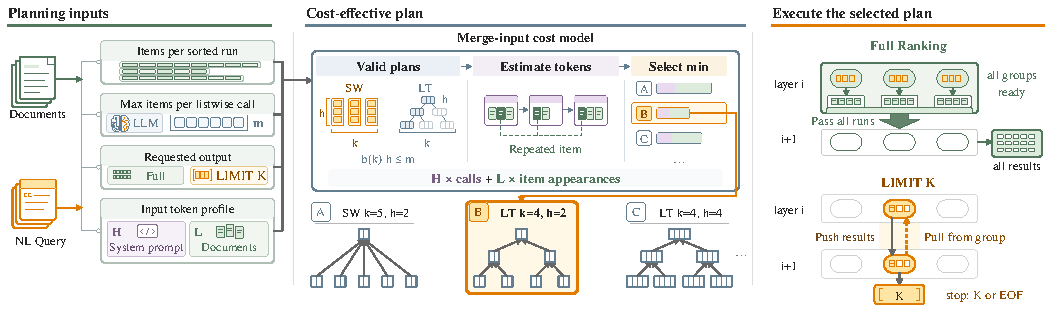
\includegraphics[width=\textwidth]{fig/mechanisms/framework.pdf}
  \caption{Cost-guided semantic \textsf{ORDER BY}. The planner compares feasible merge plans using estimated input tokens. Full ranking materializes layers; \LIMIT~$K$ requests input at group granularity. The candidate plans and token bars are schematic.}
  \label{fig:framework}
\end{figure*}


\subsection{Run Generation and Group Merge}
\label{sec:external-merge}
Algorithm~\ref{alg:semantic_external_merge} implements both phases. It partitions $D$ into $r=\lceil n/m\rceil$ disjoint chunks and ranks each chunk under the same instruction $\phi$. These calls are independent. The resulting sequences $R_1,\ldots,R_r$ are the initial runs. If there is only one run, its first $K$ items (or the whole run for Full) already answer the query.

% Paper abstraction: default no-evidence/no-shuffle path; no execution change.
{\footnotesize\raggedright
\noindent\textit{Conventions.}
$\Rank_\phi(X)$ orders real rows best first; $|X|\le1$ needs no call.
$\operatorname{take}_q$ reads the next $q$ rows or stops at exhaustion ($q=\infty$: drain).
$\Vert$ concatenates in order; $B_u$ is run $u$'s subsequence in $B$.
$\operatorname{unread}(u)$ means unread supply remains.
$\mathcal L(X)$ ranks $X$ once to order the active heads ($\rho$).
$[\bot_a]^r$ means $r$ virtual entries tagged $a$; $\operatorname{real}$ removes them.
$\MergeGroup$ forwards singletons; Full materializes each pass, LIMIT pulls and truncates only the root.
$\mathcal F$ is the feasible set; estimates use run lengths, token profile, mode and $K$.
\textsc{HalvingTree} rounds the left size up; \textsc{Cut} takes maximal subtrees within the frontier bound.\par}


\algcolstart
\begin{algorithm}[H]
\caption{External Merge Group via $k$-Way Merge}
\label{alg:semantic_external_merge}
\KwIn{rows $D$, instruction $\phi$, capacity $m$, mode Full or LIMIT, bound $K$ (default $\infty$)}
\lIf{$D=\varnothing$ or $K=0$}{\Return $[\,]$}
$\mathcal R\leftarrow[\Rank_\phi(C):C\in\operatorname{Chunks}_m(D)]$\;
\lIf{$|\mathcal R|=1$}{\Return $\operatorname{take}_K(\mathcal R_1)$}
$(f,k,h)\leftarrow\arg\min_{(f,k,h)\in\mathcal F}\widehat C_{\rm merge}(f,k,h)$\;
\While{$|\mathcal R|>1$}{
  $\mathcal G\leftarrow\operatorname{Chunks}_k(\mathcal R)$\;
  $\mathcal R'\leftarrow[\MergeGroup_{f,h}(G):G\in\mathcal G]$\;
  \lIf{Full}{$\mathcal R'\leftarrow[\operatorname{materialize}(S):S\in\mathcal R']$}
  $\mathcal R\leftarrow\mathcal R'$\;
}
\Return $\operatorname{take}_K(\mathcal R_1)$\;
\end{algorithm}
\algcolend


For multiple runs, the algorithm selects the plan once and partitions the current runs into consecutive groups of at most $k$ in each pass. Each invocation of \textsc{MergeGroup} combines one group into a run; a singleton passes through unchanged. In Full mode, groups in the same pass can execute in parallel. The next pass begins once their outputs have been materialized. Figure~\ref{fig:alg1-full-trace} illustrates this schedule for $n=16$, $m=4$, and $k=2$. Four listwise calls generate four runs. The first merge pass combines $R_1$ with $R_2$ and $R_3$ with $R_4$; the second merges the two outputs. A group merge can require several listwise calls, as the following algorithms show.

\begin{figure}\centering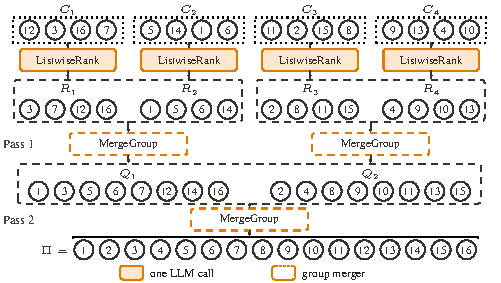
\includegraphics[width=\columnwidth]{fig/mechanisms/alg1-trace/alg1-trace.pdf}\caption{Algorithm 1, Full trace ($n=16$, $m=4$, fixed $k=2$). Four listwise calls generate runs; two merge passes reduce $4\to2\to1$ runs. MergeGroup uses SW or LT($h$) and may make multiple calls.}\label{fig:alg1-full-trace}\end{figure}


\subsection{Sliding-Window Merge}
\label{sec:sw}
SW amortizes one call over several output items by taking a short prefix from \emph{each} active run. Algorithm~\ref{alg:sliding_window_kway_group_merge} retains un-emitted items in a buffer $B$. Let $A$ contain the runs with items in $B$ or with unread input. The optimized SW plan fixes the integer quota $h$ for both Full and \textsf{LIMIT}. It refills only each run's deficit up to $h$ and leaves slots vacant when the run has too few items. When only one run remains, SW forwards its remaining items in run order without another call.

\algcolstart
\begin{algorithm}[H]
\caption{Sliding-Window Semantic $k$-Way Merge}
\label{alg:sliding_window_kway_group_merge}
\KwIn{$2\le g\le m$ runs; quota $1\le h\le\lfloor m/g\rfloor$}
$B\leftarrow[\,]$\;
\While{$B\ne[\,]$ or some run is unread}{
  $A\leftarrow\{u:|B_u|>0\ \lor\ \operatorname{unread}(u)\}$\;
  \ForEach{$u\in A$ in run order}{
    $B\leftarrow B\Vert\operatorname{take}_{\max(0,h-|B_u|)}(R_u)$\;
  }
  \lIf{$B=[\,]$}{stop}
  $A\leftarrow\{u:|B_u|>0\ \lor\ \operatorname{unread}(u)\}$\;
  \lIf{$A=\{u\}$}{yield $B_u$ then stream $R_u$ on demand; stop}
  $O\leftarrow\Rank_\phi(B)$\;
  $J\leftarrow\{j:\exists u,\ \operatorname{unread}(u),\ |B_u|>0,$\;
  \Indp $\qquad |(O_{1:j})_u|=|B_u|\}$\;\Indm
  $t\leftarrow\min(J\cup\{|O|\})$\;
  yield $O_{1:t}$; $B\leftarrow\operatorname{stableRemove}(B,O_{1:t})$\;
}
\end{algorithm}
\algcolend


\paragraph{Where to stop.}
Let $O$ be the listwise ranking of $B$. SW scans $O$ in order and emits through the first item that empties the buffered portion of a run \emph{with unread input}. The next item of that run was absent from the call and could precede the rest of $O$. A run with no unread input imposes no such boundary. If no run imposes a boundary, SW emits all of $O$. Under a common ordering of the runs and the batch, every emitted item precedes the unseen suffixes: until the boundary, each nonempty unseen suffix still has a buffered predecessor, including the boundary item itself for the run that triggers the stop. This is the sense in which the prefix is \emph{safe} (Appendix~\ref{app:proof-sw}). SW removes the emitted items from $B$, preserving the buffer order of the survivors for the next refill.

\begin{figure}[t]
  \centering
  % SVG physical metrics target this measured VLDB column width.
  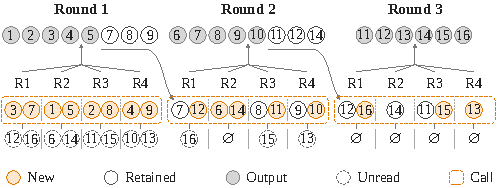
\includegraphics[width=\linewidth]{fig/mechanisms/sw.pdf}
  \caption{Sliding-window merge ($m=8$), emitting $5+5+6$ items. A prefix ends when a run with unread rows empties its window: $R_2$ at 5, then $R_4$ at 10. With nothing unread, round 3 drains the buffer. Retained items stay buffered without reordering; windows are grouped by run for display.}
  \label{fig:sw-mechanism}
\end{figure}


In Figure~\ref{fig:sw-mechanism}, four runs contribute two items each to a window of size eight. The first call places $1,2,3,4,5$ first. Item~5 consumes the last buffered item of $R_2$, but $R_2$ still holds~6. Emitting~7 from the same ranking would therefore skip~6. The second call includes~6 and emits through~10, where $R_4$ must be refilled. In the third call no run has unread input, so the remaining six items are all emitted.

\subsection{Segmented Loser-Tree Merge}
\label{sec:lt}
When SW refills even one run, it resubmits the surviving items from the whole window. LT($h$) confines each update to one path through a binary tree. Its leaves represent the $g$ runs of the group. Each internal node retains a \emph{loser segment} of at most $h$ rows and a pointer to one child. A \emph{winner segment} travels upward; at the root it becomes the next output. No other winner segments need to persist between refreshes.

\algcolstart
\begin{algorithm}[H]
\caption{Loser-Tree Semantic $k$-Way Merge}
\label{alg:loser_tree_kway_group_merge}
\KwIn{$g\ge2$ runs, $h\ge1$, $(1+\lceil\log_2 g\rceil)h\le m$}
$T\leftarrow\operatorname{HalvingTree}(R_1,\ldots,R_g)$; $F\leftarrow\operatorname{leaves}(T)$\;
\ForEach{$u\in F$}{$S_u\leftarrow\operatorname{take}_h(R_u)$}
\While{$F\ne\{\mathrm{root}\}$}{
  $\mathcal B\leftarrow\operatorname{Cut}(T,F,\lfloor m/h\rfloor)$\;
  \ForEach{$b\in\mathcal B$ with more than one frontier leaf}{
    $X\leftarrow\mathop{\Vert}_{u\in F\cap b}^{\rm left\ to\ right}S_u$;
    $\rho\leftarrow\mathcal L(X)$\;
    \ForEach{new internal $v$ of $b$, bottom-up}{
      $(S_v,\ell_v,p_v)\leftarrow\Replay(v,S_{v_L},S_{v_R},\rho)$\;
    }
  }
  $F\leftarrow\{\operatorname{root}(b):b\in\mathcal B\}$\;
}
\While{$S_{\rm root}\ne[\,]$}{yield $S_{\rm root}$; $S_{\rm root}\leftarrow\Refresh(T)$}
\end{algorithm}
\algcolend


\paragraph{Building the tree.}
Algorithm~\ref{alg:loser_tree_kway_group_merge} recursively halves the runs, giving the larger half to the left child when the count is odd. The resulting tree has exactly $g$ leaves and depth $d=\lceil\log_2 g\rceil$. Each leaf initially supplies up to $h$ items. If all $gh$ slots fit in a prompt, a single rank map suffices for bottom-up construction. Otherwise, the algorithm partitions the current frontier into maximal subtrees with at most $\lfloor m/h\rfloor$ frontier segments each. For each such subtree it ranks the real rows together, replays its internal matches using that rank map, and takes the subtree winner as one segment of the next frontier. This repeats until the root winner is available. To form a rank map $\rho$, LT preserves each input run's established order: among eligible run heads it repeatedly takes the head ranked earliest in the listwise response.

\begin{figure}[t]
  \centering
  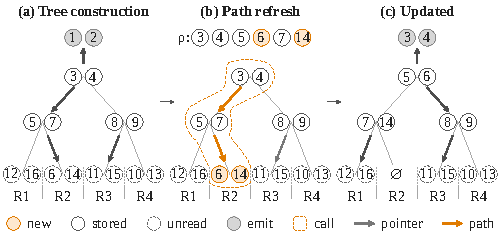
\includegraphics[width=\linewidth]{fig/mechanisms/lt.pdf}
  \caption{A refresh in a segmented loser tree ($h=2$). After the root emits $[1,2]$, the pointers lead to $R_2$. The ranker sees the replacement segment and only the losers on that path. Replaying the two matches yields $[3,4]$.}
  \label{fig:lt-mechanism}
\end{figure}


\paragraph{Choosing the next child.}
A winner segment can contain items from both children. The origin of its last item therefore does not tell us which child to refill. Algorithm~\ref{alg:replay_segment_node} makes two distinct decisions from the same ranking. It tags the two input segments as left and right \emph{slots} and orders their rows by $\rho$. The first $h$ positions supply the winner, and the remainder form the stored loser. To set the pointer, it scans the entire ranked sequence until either slot contributes its $h$-th entry. The child corresponding to that slot is the one whose next segment is needed. At a run tail, virtual entries complete each slot to length $h$ after the real rows; they affect the slot counts but never enter a prompt or an output.

\algcolstart
\begin{algorithm}[H]
\caption{Node Replay}
\label{alg:replay_segment_node}
\KwIn{node $v$, slots $s_L,s_R$ with $|s_L|,|s_R|\le h$, rank map $\rho$}
$Z\leftarrow\operatorname{sort}_\rho(s_L\Vert s_R)$, retaining slot tags\;
$Z\leftarrow Z\Vert[\bot_L]^{h-|s_L|}\Vert[\bot_R]^{h-|s_R|}$\;
$j^*\leftarrow\min\{j:\max_{a\in\{L,R\}}|(Z_{1:j})_a|=h\}$\;
$p\leftarrow v_{\operatorname{slot}(Z_{j^*})}$\;
\Return $(\operatorname{real}(Z_{1:h}),\operatorname{real}(Z_{h+1:}),p)$\;
\end{algorithm}
\algcolend

\begin{figure}[t]
  \centering
  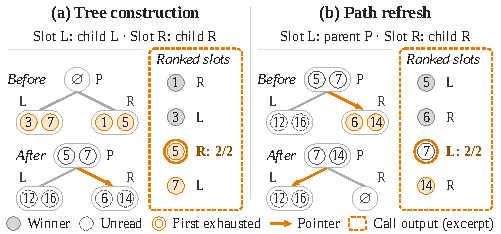
\includegraphics[width=\linewidth]{fig/mechanisms/pointer.pdf}
  \caption{Pointer assignment ($h=2$). The first slot to supply its second entry in the replay order determines the pointer. In (a), R reaches that entry at row 5. In (b), the old parent segment occupies L and reaches its second entry at row 7. L and R are slot labels, not the original run identities.}
  \label{fig:pointer-mechanism}
\end{figure}


Figure~\ref{fig:pointer-mechanism}(a) illustrates the distinction for $h=2$. The ranked slots are $1_R,3_L,5_R,7_L$. The winner is $[1,3]$, but the pointer selects the right child: its second entry is~5, before the left slot's second entry~7. The node retains $[5,7]$. These rows came from different children; at the next replay they occupy one slot together. In Figure~\ref{fig:pointer-mechanism}(b), that retained segment occupies the left slot and the incoming $[6,14]$ occupies the right. The node forwards $[5,6]$, keeps $[7,14]$, and now points left.

\paragraph{Refreshing one path.}
After the root segment has been emitted, Algorithm~\ref{alg:refresh_loser_tree_path} follows child pointers from the root to one leaf. It pulls that run's next segment and collects the loser segments stored on the path. A single listwise call ranks the collected real rows when at least two are present. The path contains at most $d$ internal nodes, so the prompt contains at most $(d+1)h$ items; this is why LT requires $(d+1)h\le m$. The algorithm replays the path bottom-up under the resulting $\rho$. At each node, the incoming segment occupies the slot named by the old pointer, and the previously stored loser occupies the other slot. Replay installs the new loser and pointer and sends the winner upward. All nodes outside the path keep their state. Even when calls disagree, this replay rule preserves the order of each input run and emits only prefixes of it (Appendix~\ref{app:proof-inconsistent}).

\algcolstart
\begin{algorithm}[H]
\caption{Path Refresh}
\label{alg:refresh_loser_tree_path}
\KwIn{LT($h$) $T$ after root emission; losers $\ell_v$ and child pointers $p_v$ at internal nodes}
$P\leftarrow[\,]$; $u\leftarrow\operatorname{root}(T)$\;
\While{$u$ is internal}{$P\leftarrow P\Vert[u]$; $u\leftarrow p_u$}
$S\leftarrow\operatorname{take}_h(R_u)$\;
$X\leftarrow S\Vert\mathop{\Vert}_{v\in P}\ell_v$; $\rho\leftarrow\mathcal L(X)$\;
\ForEach{$v\in\operatorname{reverse}(P)$}{
  $(s_L,s_R)\leftarrow(S,\ell_v)$ if $p_v=v_L$, else $(\ell_v,S)$\;
  $(S,\ell_v,p_v)\leftarrow\Replay(v,s_L,s_R,\rho)$\;
}
\Return $S$\;
\end{algorithm}
\algcolend


Figure~\ref{fig:lt-mechanism} traces one refresh on the same four runs as SW, with $h=2$. After the root emits $[1,2]$, the pointers lead to $R_2$. Its new segment $[6,14]$ joins $[5,7]$ and $[3,4]$, the two stored losers on the path. The repaired rank map orders these six rows as $[3,4,5,6,7,14]$. Two local replays produce the next root segment $[3,4]$ without another model call. The right subtree, which retains $[8,9]$, contributes no rows to this prompt.

\paragraph{The single-item case.}
Setting $h=1$ recovers the structure of the classical loser tree~\cite{DBLP:journals/csur/Graefe06}. Each node stores one loser, each nonempty root segment contains one winner, and the pointer follows the child supplying that winner. Refresh replaces one run head and replays its path. The semantic implementation still ranks the replacement and its path opponents together; the binary matches use positions in that ranking. Increasing $h$ uses the same tree and replay rule to deliver up to $h$ items per refresh.

\subsection{Demand-Driven Execution for \textsf{LIMIT}~$K$}
\label{sec:topk}\label{sec:topk-exec}
Materializing every group would compute intermediate tails that a prefix query might never read. For a prefix in the ranker's output direction, we keep run generation unchanged and execute the merge groups as producers. A leaf serves an initial run in order. An internal producer answers a request for rows first from its pending output; when it needs more, it advances its own merger. In strict-demand mode there is no background prefetch. An SW group pulls enough from each deficient child to form its window. An LT group initially pulls a segment from each child and subsequently refills only the leaf named by its pointer path. A request for even one output row can thus require several child rows or a complete listwise call. The limit applies to rows returned by the root, not to the number of rows that each child may supply.

The root stops after $K$ items or on exhaustion, and the executor closes the producer tree. It does not start a new root refresh to complete a segment after meeting the limit. For example, with $K=3$ in Figure~\ref{fig:lt-mechanism}, the root returns the initial $[1,2]$ and the first item of the next segment $[3,4]$. It then stops without following another pointer. For a fixed merge plan and identical listwise responses on the calls it reaches, this returns the prefix of the full execution of \emph{that plan}: each group consumes the same child prefixes and performs the same state transitions until the final requested item. This execution saves work on intermediate tails; we next estimate how much of that work each candidate plan avoids.

\section{Token Cost Model}
\label{sec:cost}

\subsection{Full Ranking}
\label{sec:cost-full}

A larger fan-in $k$ reduces the number of merge passes, but it also changes what each listwise call ranks. A sliding window resubmits items that remain in the window; a loser tree resubmits the segments retained along one path. The call-count proxy in Section~\ref{sec:prelim} treats prompts as having comparable footprints. The optimizer relaxes that approximation because merge prompts differ in width: it counts both calls and item appearances. Run generation is common to all plans, so only the merge cost enters plan selection.

\stitle{Pricing a request.}
For a fixed instruction and prompt template, we serialize sampled input items at several batch widths and count the input tokens in each request. We fit the token count for a request of width $b$ as $H+Lb$, where $H$ is the fixed overhead per request and $L$ is the estimated incremental length per item. For a merge plan $\theta=(f,k,h)$ with family $f$, let $A$ denote the number of listwise calls and $S=\sum_{j=1}^{A}b_j$ the number of item appearances, counting an item each time it is submitted. The resulting estimate is
\begin{equation}
  \widehat C(\theta)=H\widehat{\mathbb E}[A]+L\widehat{\mathbb E}[S].
  \label{eq:merge-cost-model}
\end{equation}
The ratio $H/L$ gives the trade-off in units of items: saving one call offsets up to $H/L$ additional item appearances.

\stitle{Estimating full-merge work.}
Let $\boldsymbol{\ell}=(\ell_1,\ldots,\ell_r)$ be the lengths of the initial runs, with $\sum_i\ell_i=n$. These lengths determine the merge groups, but not when a window must refill or which path a tree must refresh. To model this uncertainty, we distribute the ranks $1,\ldots,n$ uniformly among runs of the specified lengths and sort each run internally. This models interleaving without replacement and preserves the exact size of the last run.

On one sampled assignment $\pi$, we replay the materialized passes using integer ranks for comparisons. If $\mathcal G_t$ is the set of non-singleton groups in pass $t$ and $(A_g,S_g)$ are the counts for group $g$, then
\begin{equation}
  (A,S)_{\mathrm{full}}(\pi)=
  \sum_{t=1}^{\lceil\log_k r\rceil}
  \sum_{g\in\mathcal G_t}(A_g(\pi),S_g(\pi)).
  \label{eq:total-merge-cost}
\end{equation}
For a window, each ranked batch contributes one call and its actual occupancy; once only one run remains, it drains for free. For a loser tree, the counts include the packed initialization calls and the actual width of each path refresh, including partially filled segments. Groups in later passes receive the merged ranks from the same assignment. We average the counts over Monte Carlo assignments and cache them by plan and run lengths for each execution mode and demand. The cached counts do not depend on $H$ or $L$, so a new token profile can price the same plans without rerunning the simulation or invoking the ranker.

\stitle{Selecting a plan.}
We enumerate integer $2\leq k\leq r$ and $1\leq h\leq h_{\max}(f,k)$, where
\begin{equation}
 h_{\max}(f,k)=
 \begin{cases}
   \lfloor m/k\rfloor, & f=\mathrm{SW},\\
   \lfloor m/(1+\lceil\log_2 k\rceil)\rfloor, & f=\mathrm{LT}.
 \end{cases}
 \label{eq:merge-capacity}
\end{equation}
The first bound fits the $k$ per-run buffers in a single window; the second fits a replacement segment and the retained segments on the longest refresh path. We select the plan with the smallest estimate in Eq.~\eqref{eq:merge-cost-model}, searching within the requested family or across both families when the choice is open. If there is at most one initial run, no merge is needed.

\stitle{Position-aware pricing.}
Eq.~\eqref{eq:merge-cost-model} prices every appearance at the same mean length $L$. A long item near the head of a run can, however, appear in more prompts than a long item near its tail. We therefore distinguish the mean-length model (v5) from a position-aware variant (v6). In the same simulations, let $W_b$ be the mean number of calls of width $b$, and $E_{ip}$ the mean number of appearances of position $p$ in initial run $i$. After run generation, let $s_{ip}$ be the token length of the actual item at that position and $B_b$ the template and formatting cost for width $b$. The position-aware estimate is
\begin{equation}
  \widehat C_{\mathrm{pos}}(\theta)=
  \sum_{b=2}^{m}W_b B_b+
  \sum_{i=1}^{r}\sum_{p=1}^{\ell_i}E_{ip}s_{ip}.
  \label{eq:cost-position-aware}
\end{equation}
The widths and exposure counts are precomputed; the planner maps the measured item lengths to their observed run positions before choosing $(k,h)$.

\subsection{\texorpdfstring{\textsf{LIMIT}~$K$}{LIMIT K}}
\label{sec:cost-limit}

For a strict prefix, multiplying the full cost by $K/n$ would prorate initialization as well as refreshes. Yet the first output already requires candidates from every input run. Subsequent outputs can draw repeatedly on one subtree while another subtree continues to serve items it has buffered. Thus the cost at a child depends on which items its parent consumes.

We use the same rank assignments and token profile, but replay the producer tree under strict demand. Starting at the root, the simulation pulls only the items needed by the current window or segment. A child serves buffered output directly and requests more input when its merge state requires it. We stop when the root has returned $K$ items, charging the full width of any call that supplied them even when some of its output remains buffered. The resulting $(A_K,S_K)$ replace $(A,S)$ in Eq.~\eqref{eq:merge-cost-model}; position-aware pricing likewise uses the widths and exposures recorded up to this stopping point. For $0<K<n$, the planner searches $1\leq h\leq\min\{K,h_{\max}(f,k)\}$; a zero demand incurs no merge work.

\stitle{An exact prefix case.}
For a loser tree with $h=1$ and $1\leq K\leq\min_i\ell_i$, every replacement needed before termination is available from its source run. Initialization yields the first item. Each of the remaining $K-1$ outputs requires refreshing the path of the preceding output. Let $(a_i,d_i)$ count the calls and item appearances on that path if the preceding item came from initial run $i$, including every merge group between that run and the root. Under the finite interleaving model, each global position belongs to run $i$ with probability $\ell_i/n$. With initialization counts $(A_0,S_0)$, linearity of expectation gives
\begin{equation}
 (\mathbb E[A_K],\mathbb E[S_K])=(A_0,S_0)
  +(K-1)\sum_{i=1}^{r}\frac{\ell_i}{n}(a_i,d_i).
 \label{eq:cost-limit-single}
\end{equation}
This shortcut gives exact call and appearance means for Eq.~\eqref{eq:merge-cost-model}. The general prefix estimator and the position-specific weights in Eq.~\eqref{eq:cost-position-aware} use finite-tree simulation.

\FloatBarrier
\section{Experimental Study}
\label{sec:exp}

Sections~\ref{sec:exp:setup}--\ref{sec:exp:protocols} detail our setup across five evaluation facets:
\ding{172}~end-to-end quality, tokens, and latency on Full and \LIMIT~10 (Section~\ref{sec:exp:e1});
\ding{173}~cost-model surface fidelity and planner regret across $(k,h)$ and header ratios (Section~\ref{sec:exp:e2});
\ding{174}~scalability to $n{=}10{,}000$ (Section~\ref{sec:exp:scale});
\ding{175}~KV prefix caching and discount $\beta$ sensitivity (Section~\ref{sec:exp:cache}); and
\ding{176}~demand adaptation from small \LIMIT~$K$ to Full (Section~\ref{sec:exp:limit-sweep}).

\subsection{Experimental Setup}
\label{sec:exp:setup}

\stitle{Datasets.}
E1 spans 151 queries over six benchmarks (Table~\ref{tab:datasets}): SemBench Movie Q9~\cite{lao2026sembench} (128 reviews of one movie ranked by sentiment against rating grades), plus 30 queries each from TREC DL20~\cite{arxiv21trecdl20}, DL22~\cite{arxiv25trecdl22}, and BEIR~\cite{arxiv21BEIR} (TREC-COVID, DBpedia-Entity, Robust04). For retrieval suites, let $J_q$ count distinct judged candidates with text for query $q$; we select queries with $J_q > 100$ and at least two grades, stratified by pool size and dominant-grade share, sampling $n = \min(J_q, 500)$ proportionally when $J_q > 500$ (collapsing official equivalence classes first on DL22). Outside E1, BM25 pools use three length-stratified queries each from DL20 and TREC-COVID unless noted.

% Corpus sizes are source collection sizes, not per-query E1 input sizes.
% E1 query counts: frozen experiment.yaml and paper-delivery readiness record.
\begin{table}[t]
  \centering\small
  \caption{Source collections and query counts for E1.}
  \label{tab:datasets}
  \setlength{\tabcolsep}{3pt}
  \begin{tabular*}{\columnwidth}{@{\extracolsep{\fill}}llrlr@{}}
    \toprule
    Suite & Dataset & $|D|$ & Domain & Queries \\
    \midrule
    SemBench & Q9 & 1,375,738 & Movie reviews & 1 \\
    \midrule
    \multirow{2}{*}{TREC} & DL20 & 8,841,823 & Web passages & 30 \\
                          & DL22 & 138,364,198 & Web passages & 30 \\
    \midrule
    \multirow{3}{*}{BEIR} & TREC-COVID & 171,332 & Biomedical & 30 \\
                         & DBpedia-Entity & 4,635,922 & Wikipedia & 30 \\
                         & Robust04 & 528,155 & Newswire & 30 \\
    \bottomrule
  \end{tabular*}
\end{table}


\stitle{Baselines and Operators.}
We compare SW and LT($h$) against four OrderByLLM methods (Pointwise, External Pointwise, External Bubble, External Merge)~\cite{DBLP:journals/corr/abs-2509-00303}, ListK Sort and Tournament~\cite{DBLP:journals/corr/abs-2603-17223}, LOTUS Quicksort~\cite{DBLP:journals/pvldb/PatelJPGAGZ25}, and Setwise Heap~\cite{DBLP:conf/sigir/ZhuangZKZ24}. Table~\ref{tab:ranking-algorithms} summarizes logical calls for ten Full and nine \LIMIT~10 methods, omitting ListK Sort under \LIMIT~10 because ListK Select outputs an unordered set.

\stitle{Implementation Details.}
Both Qwen3.5-9B (2-way TP, default $m{=}20$) and Qwen3.8-27B (4-way TP, $m{=}22$ from pilot sweeps)~\cite{DBLP:journals/corr/abs-2505-09388} are served via vLLM~\cite{kwon2023efficient} at temperature zero and seed zero. OrderByLLM and ListK use window size $20$; Setwise Heap compares a parent with two children in one permutation. Full materializes each pass, while \LIMIT~$K$ pulls on demand without prefetching.

% Logical ranker calls, not measured requests or token costs.
\begin{table}[t]
  \centering\small
  \caption{Evaluated semantic ranking operators and logical LLM call complexities for Full and \LIMIT~$K$ execution.}
  \label{tab:ranking-algorithms}
  \setlength{\tabcolsep}{2.6pt}
  \begin{tabular*}{\columnwidth}{@{\extracolsep{\fill}}llcc@{}}
    \toprule
    Method & Prompt & Full & LIMIT $K$ \\
    \midrule
    Pointwise & Point & $n$ & $n$ \\
    Ext.\ Pointwise & Point & $r$ & $r$ \\
    Ext.\ Bubble & List & $O(r^2)$ & $O(r\lceil K/m\rceil)$ \\
    Ext.\ Merge & List & $O(r[1+\log_2 r])$ & $O(r[1+\log_2^+(K/m)])$ \\
    \midrule
    ListK Sort & List & $O(n\log n/\chi_p+n)^{*}$ & Not evaluated \\
    Tournament & List & $C_{\mathrm{tour}}(n)$ & $C_{\mathrm{tour}}(K)$ \\
    \midrule
    LOTUS Quick & Pair & $O(n\log n)^{*}$ & $O(n+K\log K)^{*}$ \\
    Setwise Heap & Set & $O(n\log n)$ & $O(n+K\log n)$ \\
    \midrule
    \SW{} & List & $r+A_{\SW{}}$ & $r+A_{\SW{},K}$ \\
    \LT($h$) & List & $r+A_{\LT{}}$ & $r+A_{\LT{},K}$ \\
    \bottomrule
  \end{tabular*}\par\smallskip
  {\raggedright\footnotesize
  $n$ is the input size, $m$ the batch capacity of the method, and $r=\lceil n/m\rceil$.
  $\log_2^+(x)=\max(0,\log_2 x)$; $\chi_p=(m-p)\log(p+1)$ for $p$ pivots.
  $C_{\mathrm{tour}}(q)$ counts tournament calls until $q$ outputs.
  $A_f$ and $A_{f,K}$ count Full and on-demand merge calls, respectively
  (Section~\ref{sec:cost}). $^{*}$ denotes expected costs under the source pivot models. Counts exclude retries, calibration, and profiling.\par}
\end{table}


\subsection{Experiment-Specific Settings}
\label{sec:exp:protocols}

\stitle{End-to-end ranking (E1).}
Full uses Spearman's $\rho$ (midranks for ties) and \LIMIT~10 uses nDCG@10 (gain $2^g - 1$). Across ten shared input permutations (seeds $0$--$9$), we average quality over queries per dataset and report mean $\pm$ SD across the ten dataset means. Quality/token runs allow ten concurrent queries and count all Input + Output tokens (including Phase~1). Isolated latency uses seed~$0$, one active query, and up to 256 concurrent requests, timing profiling through output return. Token columns sum dataset means for Q9, TREC, and BEIR; latency averages all six datasets equally, and $Q$, $T$, $L$ rank methods by mean within-dataset rank.

\stitle{Cost prediction (E2).}
E2 compares predicted and measured merge input tokens across fixed $(k,h)$ grids on two 500-candidate base workloads: DL20 (query 1109707, 9B) and TREC-COVID (query 38, 27B) under Full and \LIMIT~10. Surface agreement evaluates prediction accuracy; the gap between the planner's pick and the empirical grid minimum measures decision regret. Two padded-instruction workloads on DL20 query 1109707 (Full on 9B, $n{=}641$; \LIMIT~2 on 27B, $n{=}500$) vary fixed header $H$ at fixed item texts $L$.

\stitle{Input size (E3).}
E3 scales $n$ across $1{,}000$, $5{,}000$, and $10{,}000$ on 9B DL20 using nested samples anchored at the BM25 top 1,000, holding five $(k,h)$ pairs per family fixed (Figure~\ref{fig:e3-scale}; four extra LT pairs at larger sizes are omitted from the plot).

\Needspace{5\baselineskip}
\stitle{Prefix caching (E4).}
On 9B, with input tokens $U$, shared-prefix cache hits $Q$, and price factor $\beta \in [0,1]$, equivalent input cost is $C_\beta = U - (1-\beta)Q$ ($U$ when Off; isolated cold namespace per sort when On). E4a compares Off and On-cold ($\beta{=}0$) at $n \in \{100, 500\}$ on medium-length DL20 and COVID queries over eight evenly spaced $(k,h)$ pairs, pooling savings $100(1 - \sum_q C_{0,q}^{\mathrm{On}} / \sum_q U_q^{\mathrm{Off}})$ in Figure~\ref{fig:e4a-c2}. On DL20 ($n{=}500$, LT Full), E4b reprices seven configurations across $\beta \in \{0,.1,.25,.5,.75,.9,1\}$ (five shown in Figure~\ref{fig:e4b-beta}).

\stitle{Output size (E5).}
Across the six BM25 pools at $n{=}500$ on 9B, E5 varies $K$ over $10, 20, 50, 100, 200, 300, 400, 490$, and $500$ alongside Full under Off and On-cold ($\beta{=}0$), selecting $(k,h)$ per demand and cache state to track $C_0$ and nDCG@10 (unjudged gain zero); comparing \LIMIT~500 with Full isolates pass-materialization overhead.

\noindent\textit{Layout review copy.} The results tables and plots contain illustrative values, not experimental measurements.
% E1 through E5: results prose intentionally empty.
% Group the E1/E2 draft assets on one dedicated full-width float page.
\FloatBarrier
\begin{figure*}[p]
  \begingroup
  \renewenvironment{table*}[1][]{%
    \noindent\begin{minipage}{\textwidth}\captionsetup{type=table}\centering
  }{\end{minipage}\par\vskip1pt}%
  \renewenvironment{figure*}[1][]{%
    \noindent\begin{minipage}{\textwidth}\captionsetup{type=figure}\centering
  }{\end{minipage}\par\vskip1pt}%
\subsection{End-to-End Ranking}
\label{sec:exp:e1}
% Synthetic layout preview from round2/tables-pseudocode/src/synthetic.py.
% Single full-width 27-column dual-model table with uncrowded typography & Ours row highlight.
\begin{table*}[t]
\centering
\caption{End-to-end Full ranking quality (Spearman's $\rho\uparrow$), total tokens ($\times 10^{3}\downarrow$), and isolated latency ($\text{s}\downarrow$) across six benchmarks.}
\label{tab:exp1-full}
\begingroup
\normalfont\rmfamily\fontsize{6.4}{8.3}\selectfont
\renewcommand{\qpm}[2]{\mbox{\IfBeginWith{#1}{0.}{\StrGobbleLeft{#1}{1}}{#1}\kern0.35pt{\normalfont\textcolor[HTML]{64748B}{\fontsize{4.8}{5.8}\selectfont\textpm\IfBeginWith{#2}{0.}{\StrGobbleLeft{#2}{1}}{#2}}}}}
\setlength{\tabcolsep}{0pt}
\renewcommand{\arraystretch}{0.96}
\begin{tabular*}{\textwidth}{@{\extracolsep{\fill}}l!{\hspace{2.2pt}}c!{\hspace{1.6pt}}c!{\hspace{1.6pt}}c!{\hspace{1.6pt}}c!{\hspace{1.6pt}}c!{\hspace{1.6pt}}c!{\hspace{2.6pt}}c!{\hspace{1.5pt}}c!{\hspace{1.5pt}}c!{\hspace{2.4pt}}c!{\hspace{2.4pt}}c!{\hspace{1.1pt}}c!{\hspace{1.1pt}}c!{\hspace{3.6pt}\color[HTML]{CBD5E1}\vrule width 0.55pt\hspace{3.6pt}}c!{\hspace{1.6pt}}c!{\hspace{1.6pt}}c!{\hspace{1.6pt}}c!{\hspace{1.6pt}}c!{\hspace{1.6pt}}c!{\hspace{2.6pt}}c!{\hspace{1.5pt}}c!{\hspace{1.5pt}}c!{\hspace{2.4pt}}c!{\hspace{2.4pt}}c!{\hspace{1.1pt}}c!{\hspace{1.1pt}}c@{}}
\toprule
& \multicolumn{13}{c}{\fontsize{7.2}{8.2}\selectfont\textbf{\textcolor[HTML]{1F5A8A}{Qwen3.5-9B}}} & \multicolumn{13}{c}{\fontsize{7.2}{8.2}\selectfont\textbf{\textcolor[HTML]{A63A50}{Qwen3.8-27B}}} \\
\cmidrule(lr){2-14}\cmidrule(lr){15-27}
\textbf{Method} & \multicolumn{6}{c}{Quality $\rho\uparrow$} & \multicolumn{3}{c}{Tokens ($\times 10^{3}$)$\downarrow$} & Lat.$\downarrow$ & \multicolumn{3}{c}{Rank$\downarrow$} & \multicolumn{6}{c}{Quality $\rho\uparrow$} & \multicolumn{3}{c}{Tokens ($\times 10^{3}$)$\downarrow$} & Lat.$\downarrow$ & \multicolumn{3}{c}{Rank$\downarrow$} \\
\cmidrule(lr){2-7}\cmidrule(lr){8-10}\cmidrule(lr){12-14}\cmidrule(lr){15-20}\cmidrule(lr){21-23}\cmidrule(lr){25-27}
& Q9 & DL20 & DL22 & COVID & DBP & R04 & Q9 & TREC & BEIR & s & $Q$ & $T$ & $L$ & Q9 & DL20 & DL22 & COVID & DBP & R04 & Q9 & TREC & BEIR & s & $Q$ & $T$ & $L$ \\
\midrule
Pointwise & \underline{\qpm{0.820}{0.012}} & \underline{\qpm{0.820}{0.012}} & \underline{\qpm{0.820}{0.012}} & \textbf{\qpm{0.840}{0.012}} & \textbf{\qpm{0.840}{0.012}} & \textbf{\qpm{0.840}{0.012}} & \textbf{1.00} & \textbf{2.03} & \textbf{3.12} & \textbf{1.75} & \textbf{1} & \textbf{1} & \textbf{1} & \underline{\qpm{0.840}{0.012}} & \underline{\qpm{0.840}{0.012}} & \underline{\qpm{0.840}{0.012}} & \textbf{\qpm{0.860}{0.012}} & \textbf{\qpm{0.860}{0.012}} & \textbf{\qpm{0.860}{0.012}} & \textbf{5.00} & \textbf{10.03} & \textbf{15.12} & \textbf{2.25} & \textbf{1} & \textbf{1} & \textbf{1} \\
Ext.\ Point. & \textbf{\qpm{0.840}{0.013}} & \textbf{\qpm{0.840}{0.013}} & \textbf{\qpm{0.840}{0.013}} & \underline{\qpm{0.820}{0.013}} & \underline{\qpm{0.820}{0.013}} & \qpm{0.800}{0.013} & \underline{1.10} & \underline{2.23} & \underline{3.42} & \underline{2.15} & \underline{2} & \underline{2} & \underline{2} & \textbf{\qpm{0.860}{0.013}} & \textbf{\qpm{0.860}{0.013}} & \textbf{\qpm{0.860}{0.013}} & \underline{\qpm{0.840}{0.013}} & \underline{\qpm{0.840}{0.013}} & \qpm{0.820}{0.013} & \underline{5.10} & \underline{10.23} & \underline{15.42} & \underline{2.65} & \underline{2} & \underline{2} & \underline{2} \\
Ext.\ Bubble & \qpm{0.800}{0.014} & \qpm{0.800}{0.014} & \qpm{0.800}{0.014} & \qpm{0.800}{0.014} & \qpm{0.780}{0.014} & \underline{\qpm{0.820}{0.014}} & 1.20 & 2.43 & 3.72 & 2.55 & 3 & 3 & 3 & \qpm{0.820}{0.014} & \qpm{0.820}{0.014} & \qpm{0.820}{0.014} & \qpm{0.820}{0.014} & \qpm{0.800}{0.014} & \underline{\qpm{0.840}{0.014}} & 5.20 & 10.43 & 15.72 & 3.05 & 3 & 3 & 3 \\
Ext.\ Merge & \qpm{0.780}{0.015} & \qpm{0.780}{0.015} & \qpm{0.780}{0.015} & \qpm{0.780}{0.015} & \qpm{0.800}{0.015} & \qpm{0.780}{0.015} & 1.30 & 2.63 & 4.02 & 2.95 & 4 & 4 & 4 & \qpm{0.800}{0.015} & \qpm{0.800}{0.015} & \qpm{0.800}{0.015} & \qpm{0.800}{0.015} & \qpm{0.820}{0.015} & \qpm{0.800}{0.015} & 5.30 & 10.63 & 16.02 & 3.45 & 4 & 4 & 4 \\
\midrule
ListK Sort & \qpm{0.760}{0.016} & \qpm{0.760}{0.016} & \qpm{0.760}{0.016} & \qpm{0.760}{0.016} & \qpm{0.760}{0.016} & \qpm{0.760}{0.016} & 1.40 & 3.10 & 6.00 & 3.35 & 5 & 6 & 5 & \qpm{0.780}{0.016} & \qpm{0.780}{0.016} & \qpm{0.780}{0.016} & \qpm{0.780}{0.016} & \qpm{0.780}{0.016} & \qpm{0.780}{0.016} & 5.40 & 11.10 & 18.00 & 3.85 & 5 & 6 & 5 \\
Tournament & \qpm{0.740}{0.017} & \qpm{0.740}{0.017} & \qpm{0.740}{0.017} & \qpm{0.740}{0.017} & \qpm{0.740}{0.017} & \qpm{0.740}{0.017} & 1.41 & 3.12 & 5.10 & 3.75 & 6 & 5 & 6 & \qpm{0.760}{0.017} & \qpm{0.760}{0.017} & \qpm{0.760}{0.017} & \qpm{0.760}{0.017} & \qpm{0.760}{0.017} & \qpm{0.760}{0.017} & 5.41 & 11.12 & 17.10 & 4.25 & 6 & 5 & 6 \\
\midrule
LOTUS Quick & \qpm{0.720}{0.018} & \qpm{0.720}{0.018} & \qpm{0.720}{0.018} & \qpm{0.720}{0.018} & \qpm{0.720}{0.018} & \qpm{0.720}{0.018} & 3.00 & 6.03 & 9.12 & 4.15 & 7 & 7 & 7 & \qpm{0.740}{0.018} & \qpm{0.740}{0.018} & \qpm{0.740}{0.018} & \qpm{0.740}{0.018} & \qpm{0.740}{0.018} & \qpm{0.740}{0.018} & 7.00 & 14.03 & 21.12 & 4.65 & 7 & 7 & 7 \\
\midrule
Setwise Heap & \qpm{0.700}{0.019} & \qpm{0.700}{0.019} & \qpm{0.700}{0.019} & \qpm{0.700}{0.019} & \qpm{0.700}{0.019} & \qpm{0.700}{0.019} & 3.10 & 6.23 & 9.42 & 4.55 & 8 & 8 & 8 & \qpm{0.720}{0.019} & \qpm{0.720}{0.019} & \qpm{0.720}{0.019} & \qpm{0.720}{0.019} & \qpm{0.720}{0.019} & \qpm{0.720}{0.019} & 7.10 & 14.23 & 21.42 & 5.05 & 8 & 8 & 8 \\
\midrule
\rowcolor[HTML]{EEF4FA}\textbf{SW} & \qpm{0.680}{0.020} & \qpm{0.670}{0.030} & \qpm{0.680}{0.020} & \qpm{0.680}{0.020} & \qpm{0.680}{0.020} & \qpm{0.680}{0.020} & 3.20 & 6.43 & 9.72 & 4.95 & 9 & 9 & 9 & \qpm{0.700}{0.020} & \qpm{0.690}{0.030} & \qpm{0.700}{0.020} & \qpm{0.700}{0.020} & \qpm{0.700}{0.020} & \qpm{0.700}{0.020} & 7.20 & 14.43 & 21.72 & 5.45 & 9 & 9 & 9 \\
\rowcolor[HTML]{EEF4FA}\textbf{LT($h$)} & \qpm{0.660}{0.021} & \qpm{0.670}{0.011} & \qpm{0.660}{0.021} & \qpm{0.660}{0.021} & \qpm{0.660}{0.021} & \qpm{0.660}{0.021} & 3.30 & 6.63 & 10.02 & 5.35 & 10 & 10 & 10 & \qpm{0.680}{0.021} & \qpm{0.690}{0.011} & \qpm{0.680}{0.021} & \qpm{0.680}{0.021} & \qpm{0.680}{0.021} & \qpm{0.680}{0.021} & 7.30 & 14.63 & 22.02 & 5.85 & 10 & 10 & 10 \\
\bottomrule
\end{tabular*}
\endgroup
\end{table*}

% Synthetic layout preview from round2/tables-pseudocode/src/synthetic.py.
% LIMIT omits ListK Select; places are recomputed over the displayed methods.
\begin{table*}[t]
\centering
\caption{End-to-end \LIMIT~$K{=}10$ prefix quality (nDCG@10), total tokens ($\times 10^{3}$), and isolated latency across six benchmarks.}
\label{tab:exp1-limit}
\begingroup
\normalfont\rmfamily\fontsize{6.5}{8.2}\selectfont
\renewcommand{\qpm}[2]{\mbox{\IfBeginWith{#1}{0.}{\StrGobbleLeft{#1}{1}}{#1}{\fontsize{5.3}{6.5}\selectfont\textpm\IfBeginWith{#2}{0.}{\StrGobbleLeft{#2}{1}}{#2}}}}
\setlength{\tabcolsep}{0.15pt}
\renewcommand{\arraystretch}{0.90}
\begin{tabular*}{\textwidth}{@{\extracolsep{\fill}}l!{\hspace{1.35pt}}c!{\hspace{0.35pt}}c!{\hspace{0.35pt}}c!{\hspace{0.35pt}}c!{\hspace{0.35pt}}c!{\hspace{0.35pt}}c!{\hspace{1.35pt}}c!{\hspace{0.35pt}}c!{\hspace{0.35pt}}c!{\hspace{1.35pt}}c!{\hspace{1.35pt}}c!{\hspace{0.35pt}}c!{\hspace{0.35pt}}c!{\hspace{2.5pt}}c!{\hspace{0.35pt}}c!{\hspace{0.35pt}}c!{\hspace{0.35pt}}c!{\hspace{0.35pt}}c!{\hspace{0.35pt}}c!{\hspace{1.35pt}}c!{\hspace{0.35pt}}c!{\hspace{0.35pt}}c!{\hspace{1.35pt}}c!{\hspace{1.35pt}}c!{\hspace{0.35pt}}c!{\hspace{0.35pt}}c@{}}
\toprule
& \multicolumn{13}{c}{\fontsize{7}{8}\selectfont\textbf{Qwen3.5-9B}} & \multicolumn{13}{c}{\fontsize{7}{8}\selectfont\textbf{Qwen3.8-27B}} \\
\cmidrule(lr){2-14}\cmidrule(lr){15-27}
Method & \multicolumn{6}{c}{nDCG@10} & \multicolumn{3}{c}{Tokens $\times 10^{3}$} & Lat. & \multicolumn{3}{c}{Rank} & \multicolumn{6}{c}{nDCG@10} & \multicolumn{3}{c}{Tokens $\times 10^{3}$} & Lat. & \multicolumn{3}{c}{Rank} \\
\cmidrule(lr){2-7}\cmidrule(lr){8-10}\cmidrule(lr){12-14}\cmidrule(lr){15-20}\cmidrule(lr){21-23}\cmidrule(lr){25-27}
& Q9 & DL20 & DL22 & COVID & DBP & R04 & Q9 & TREC & BEIR & s & $Q$ & $T$ & $L$ & Q9 & DL20 & DL22 & COVID & DBP & R04 & Q9 & TREC & BEIR & s & $Q$ & $T$ & $L$ \\
\midrule
Pointwise & \underline{\qpm{0.780}{0.012}} & \underline{\qpm{0.780}{0.012}} & \underline{\qpm{0.780}{0.012}} & \textbf{\qpm{0.800}{0.012}} & \textbf{\qpm{0.800}{0.012}} & \textbf{\qpm{0.800}{0.012}} & \textbf{1.70} & \textbf{3.43} & \textbf{5.22} & \textbf{2.05} & \textbf{1} & \textbf{1} & \textbf{1} & \underline{\qpm{0.800}{0.012}} & \underline{\qpm{0.800}{0.012}} & \underline{\qpm{0.800}{0.012}} & \textbf{\qpm{0.820}{0.012}} & \textbf{\qpm{0.820}{0.012}} & \textbf{\qpm{0.820}{0.012}} & \textbf{5.70} & \textbf{11.43} & \textbf{17.22} & \textbf{2.55} & \textbf{1} & \textbf{1} & \textbf{1} \\
Ext. Pointwise & \textbf{\qpm{0.800}{0.013}} & \textbf{\qpm{0.800}{0.013}} & \textbf{\qpm{0.800}{0.013}} & \underline{\qpm{0.780}{0.013}} & \underline{\qpm{0.780}{0.013}} & \qpm{0.760}{0.013} & \underline{1.80} & \underline{3.63} & \underline{5.52} & \underline{2.45} & \underline{2} & \underline{2} & \underline{2} & \textbf{\qpm{0.820}{0.013}} & \textbf{\qpm{0.820}{0.013}} & \textbf{\qpm{0.820}{0.013}} & \underline{\qpm{0.800}{0.013}} & \underline{\qpm{0.800}{0.013}} & \qpm{0.780}{0.013} & \underline{5.80} & \underline{11.63} & \underline{17.52} & \underline{2.95} & \underline{2} & \underline{2} & \underline{2} \\
Ext. Bubble & \qpm{0.760}{0.014} & \qpm{0.760}{0.014} & \qpm{0.760}{0.014} & \qpm{0.760}{0.014} & \qpm{0.740}{0.014} & \underline{\qpm{0.780}{0.014}} & 1.90 & 3.83 & 5.82 & 2.85 & 3 & 3 & 3 & \qpm{0.780}{0.014} & \qpm{0.780}{0.014} & \qpm{0.780}{0.014} & \qpm{0.780}{0.014} & \qpm{0.760}{0.014} & \underline{\qpm{0.800}{0.014}} & 5.90 & 11.83 & 17.82 & 3.35 & 3 & 3 & 3 \\
Ext. Merge & \qpm{0.740}{0.015} & \qpm{0.740}{0.015} & \qpm{0.740}{0.015} & \qpm{0.740}{0.015} & \qpm{0.760}{0.015} & \qpm{0.740}{0.015} & 2.00 & 4.03 & 6.12 & 3.25 & 4 & 4 & 4 & \qpm{0.760}{0.015} & \qpm{0.760}{0.015} & \qpm{0.760}{0.015} & \qpm{0.760}{0.015} & \qpm{0.780}{0.015} & \qpm{0.760}{0.015} & 6.00 & 12.03 & 18.12 & 3.75 & 4 & 4 & 4 \\
\midrule
Tournament & \qpm{0.700}{0.017} & \qpm{0.700}{0.017} & \qpm{0.700}{0.017} & \qpm{0.700}{0.017} & \qpm{0.700}{0.017} & \qpm{0.700}{0.017} & 2.11 & 4.52 & 7.20 & 4.05 & 5 & 5 & 5 & \qpm{0.720}{0.017} & \qpm{0.720}{0.017} & \qpm{0.720}{0.017} & \qpm{0.720}{0.017} & \qpm{0.720}{0.017} & \qpm{0.720}{0.017} & 6.11 & 12.52 & 19.20 & 4.55 & 5 & 5 & 5 \\
\midrule
Lotus Quick & \qpm{0.680}{0.018} & \qpm{0.680}{0.018} & \qpm{0.680}{0.018} & \qpm{0.680}{0.018} & \qpm{0.680}{0.018} & \qpm{0.680}{0.018} & 3.70 & 7.43 & 11.22 & 4.45 & 6 & 6 & 6 & \qpm{0.700}{0.018} & \qpm{0.700}{0.018} & \qpm{0.700}{0.018} & \qpm{0.700}{0.018} & \qpm{0.700}{0.018} & \qpm{0.700}{0.018} & 7.70 & 15.43 & 23.22 & 4.95 & 6 & 6 & 6 \\
\midrule
Setwise Heap & \qpm{0.660}{0.019} & \qpm{0.660}{0.019} & \qpm{0.660}{0.019} & \qpm{0.660}{0.019} & \qpm{0.660}{0.019} & \qpm{0.660}{0.019} & 3.80 & 7.63 & 11.52 & 4.85 & 7 & 7 & 7 & \qpm{0.680}{0.019} & \qpm{0.680}{0.019} & \qpm{0.680}{0.019} & \qpm{0.680}{0.019} & \qpm{0.680}{0.019} & \qpm{0.680}{0.019} & 7.80 & 15.63 & 23.52 & 5.35 & 7 & 7 & 7 \\
\midrule
SW & \qpm{0.640}{0.020} & \qpm{0.630}{0.030} & \qpm{0.640}{0.020} & \qpm{0.640}{0.020} & \qpm{0.640}{0.020} & \qpm{0.640}{0.020} & 3.90 & 7.83 & 11.82 & 5.25 & 8 & 8 & 8 & \qpm{0.660}{0.020} & \qpm{0.650}{0.030} & \qpm{0.660}{0.020} & \qpm{0.660}{0.020} & \qpm{0.660}{0.020} & \qpm{0.660}{0.020} & 7.90 & 15.83 & 23.82 & 5.75 & 8 & 8 & 8 \\
LT($h$) & \qpm{0.620}{0.021} & \qpm{0.630}{0.011} & \qpm{0.620}{0.021} & \qpm{0.620}{0.021} & \qpm{0.620}{0.021} & \qpm{0.620}{0.021} & 4.00 & 8.03 & 12.12 & 5.65 & 9 & 9 & 9 & \qpm{0.640}{0.021} & \qpm{0.650}{0.011} & \qpm{0.640}{0.021} & \qpm{0.640}{0.021} & \qpm{0.640}{0.021} & \qpm{0.640}{0.021} & 8.00 & 16.03 & 24.12 & 6.15 & 9 & 9 & 9 \\
\bottomrule
\end{tabular*}
\endgroup
\end{table*}


\subsection{Cost Model}
\label{sec:exp:e2}
{\graphicspath{{fig/experiments/fig06-cost-model/}}%
% E2. Twelve independent PDFs + single-row shared legend. Full width: 504.4bp.
% Six at 83.15bp leave room for regular flexible gutters; no negative overlap.
\newcommand{\eTwoDiamond}{\makebox[3.48bp][c]{\raisebox{0.2bp}{\includegraphics[width=4.2bp]{e2-role-diamond.pdf}}}}
% Anchor the annotations on the upper-right pane of the projected 3-D box.
% Distances are in the unchanged 83.15 bp panel, measured from top/right.
\newsavebox{\eTwoPanelGraphic}
\newcommand{\eTwoInteriorRow}[2]{%
  \makebox[0pt][r]{%
    \raisebox{\dimexpr\ht\eTwoPanelGraphic-#1\relax}[0pt][0pt]{%
      \fontsize{6.2bp}{7bp}\selectfont\makebox[22.3bp][l]{#2}}%
    \kern19.96bp}}
\newcommand{\eTwoAnnotated}[3]{%
  \begin{minipage}{83.15bp}\centering
    \sbox{\eTwoPanelGraphic}{\includegraphics[width=\linewidth,trim=4.05bp 2.2bp 1.35bp 3.2bp,clip]{#1}}%
    \usebox{\eTwoPanelGraphic}%
    \eTwoInteriorRow{26.89bp}{#2}%
    \eTwoInteriorRow{33.77bp}{#3}%
  \end{minipage}}

\begin{figure*}[t]
\centering
\setlength{\subfigtopskip}{1pt}\setlength{\subfigcapskip}{1pt}\setlength{\subfigbottomskip}{1pt}
\includegraphics[width=325bp]{e2-legend.pdf}\par
\subfigure[Syn-A, LT, Full]{\eTwoAnnotated{panels/p01.pdf}{\textcolor[HTML]{087F9B}{\ding{72}} (13,1)}{\textcolor[HTML]{DA821E}{\eTwoDiamond} (22,1)}}\hfill%
\subfigure[Syn-B, LT, Full]{\eTwoAnnotated{panels/p02.pdf}{\textcolor[HTML]{087F9B}{\ding{72}} (15,1)}{\textcolor[HTML]{DA821E}{\eTwoDiamond} (6,1)}}\hfill%
\subfigure[Syn-C, LT, Full]{\eTwoAnnotated{panels/p03.pdf}{\textcolor[HTML]{087F9B}{\ding{72}}\kern0.9bp\textcolor[HTML]{DA821E}{\eTwoDiamond} (8,1)}{}}\hfill%
\subfigure[Syn-D, LT, \textsf{LIMIT}~10]{\eTwoAnnotated{panels/p04.pdf}{\textcolor[HTML]{087F9B}{\ding{72}} (12,1)}{\textcolor[HTML]{DA821E}{\eTwoDiamond} (2,10)}}\hfill%
\subfigure[Syn-E, LT, \textsf{LIMIT}~10]{\eTwoAnnotated{panels/p05.pdf}{\textcolor[HTML]{087F9B}{\ding{72}} (7,1)}{\textcolor[HTML]{DA821E}{\eTwoDiamond} (13,1)}}\hfill%
\subfigure[Syn-F, LT, \textsf{LIMIT}~10]{\eTwoAnnotated{panels/p06.pdf}{\textcolor[HTML]{087F9B}{\ding{72}} (19,1)}{\textcolor[HTML]{DA821E}{\eTwoDiamond} (14,2)}}\par
\vspace{4.5bp}
\subfigure[Syn-G, SW, Full]{\eTwoAnnotated{panels/p07.pdf}{\textcolor[HTML]{087F9B}{\ding{72}} (6,1)}{\textcolor[HTML]{DA821E}{\eTwoDiamond} (11,1)}}\hfill%
\subfigure[Syn-H, SW, Full]{\eTwoAnnotated{panels/p08.pdf}{\textcolor[HTML]{087F9B}{\ding{72}} (11,1)}{\textcolor[HTML]{DA821E}{\eTwoDiamond} (6,2)}}\hfill%
\subfigure[Syn-I, SW, Full]{\eTwoAnnotated{panels/p09.pdf}{\textcolor[HTML]{087F9B}{\ding{72}}\kern0.9bp\textcolor[HTML]{DA821E}{\eTwoDiamond} (9,1)}{}}\hfill%
\subfigure[Syn-J, SW, \textsf{LIMIT}~10]{\eTwoAnnotated{panels/p10.pdf}{\textcolor[HTML]{087F9B}{\ding{72}} (9,1)}{\textcolor[HTML]{DA821E}{\eTwoDiamond} (2,10)}}\hfill%
\subfigure[Syn-K, SW, \textsf{LIMIT}~10]{\eTwoAnnotated{panels/p11.pdf}{\textcolor[HTML]{087F9B}{\ding{72}} (12,1)}{\textcolor[HTML]{DA821E}{\eTwoDiamond} (20,1)}}\hfill%
\subfigure[Syn-L, SW, \textsf{LIMIT}~10]{\eTwoAnnotated{panels/p12.pdf}{\textcolor[HTML]{087F9B}{\ding{72}} (18,1)}{\textcolor[HTML]{DA821E}{\eTwoDiamond} (14,1)}}\par
\caption{Front axis $k$ (fan-in), depth axis $h$ (SW per-run quota; LT segment length); vertical merge input tokens $\times 10^{3}$. Vertical ranges adapt per panel; compare numeric ticks, not apparent heights across panels. Stars mark illustrative minima over shown configurations; hollow diamonds mark model-selected configurations at the illustrative reference cost.}
\label{fig:e2-surface-exp5-12}
\end{figure*}
}

  \endgroup
\end{figure*}
% E3 is a single row across both columns; E4a and E4b below are single-column figures.
\twocolumn[{%
\begin{minipage}{\textwidth}
  \begingroup
  \renewenvironment{figure*}[1][]{\par\centering\captionsetup{type=figure}}{\par}%
  \subsection{Large-Scale Ranking}
  \label{sec:exp:scale}
  % E3: selected 1x4 overlay, with native subfigure captions and vector panels.
\begin{figure}[t]
\setlength{\subfigcapskip}{1pt}\setlength{\subfigtopskip}{0pt}\setlength{\subfigbottomskip}{1pt}
\centering
\includegraphics[width=\columnwidth]{config-legend.pdf}\par
\includegraphics[width=\columnwidth]{kind-legend.pdf}\par
\subfigure[SW, Full]{\includegraphics[width=.274716\columnwidth]{overlay-sw-full.pdf}}%
\subfigure[SW, LIMIT]{\includegraphics[width=.241761333\columnwidth]{overlay-sw-limit10.pdf}}%
\subfigure[LT, Full]{\includegraphics[width=.241761333\columnwidth]{overlay-lt-full.pdf}}%
\subfigure[LT, LIMIT]{\includegraphics[width=.241761333\columnwidth]{overlay-lt-limit10.pdf}}
\caption{Scale scaffold. Predicted (dashed, hollow) and Reference (solid, filled) share each panel. Colors and marker shapes retain fixed $(k,h)$ configurations; SW first five, LT last five. Shared axes: linear input size $n$ and synthetic layout units, not tokens or time. Full and LIMIT reuse fixture curves; offsets are not prediction error.}
\label{fig:e3-scale}
\end{figure}

  \endgroup
\end{minipage}\par\vspace{4pt}%
}]
\begingroup
\placeexperimentfigures
\subsection{Prefix Cache}
\label{sec:exp:cache}
% E4a display domain. The experimental collection contract is unchanged.
\begin{figure}[t]
\centering
% Independent vector panels. LaTeX owns the subfigure labels and captions.
\begingroup

% Center native captions under the colored grids, not the boxes including axes.
\makeatletter
\let\EfourOriginalCaption\@makesubfigurecaption
\def\@makesubfigurecaption#1#2{\hbox{\kern5bp\EfourOriginalCaption{#1}{#2}\kern-5bp}}
\makeatother
\setlength{\subfigtopskip}{0pt}
\setlength{\subfigcapskip}{1pt}
\setlength{\subfigbottomskip}{0pt}
\leavevmode\vbox{\offinterlineskip
  \hbox to \linewidth{\hfil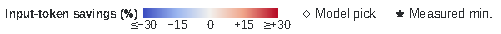
\includegraphics[width=\linewidth]{fig/experiments/fig08-cache-savings/fig08-cache-savings-color-key.pdf}\hfil}%
  \kern2bp
  \hbox to \linewidth{\hfil
    \subfigure[SW, Full]{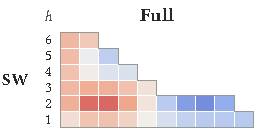
\includegraphics[width=.486\linewidth,trim=0bp 0bp 16bp 3.5bp,clip=false]{fig/experiments/fig08-cache-savings/fig08-cache-savings-a-sw-full.pdf}\label{fig:e4a-sw-full}}%
    \hspace{3.5bp}%
    \subfigure[SW, \textsf{LIMIT}~10]{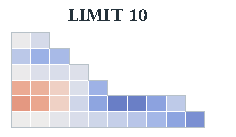
\includegraphics[width=.486\linewidth,trim=0bp 0bp 16bp 3.5bp,clip=false]{fig/experiments/fig08-cache-savings/fig08-cache-savings-c-sw-limit10.pdf}\label{fig:e4a-sw-topk}}%
    \hfil
  }%
  \kern3bp
  \hbox to \linewidth{\hfil
    \subfigure[LT, Full]{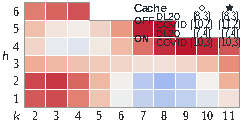
\includegraphics[width=.486\linewidth,trim=0bp 0bp 16bp 3.5bp,clip=false]{fig/experiments/fig08-cache-savings/fig08-cache-savings-b-lt-full.pdf}\label{fig:e4a-lt-full}}%
    \hspace{3.5bp}%
    \subfigure[LT, \textsf{LIMIT}~10]{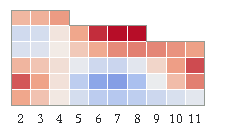
\includegraphics[width=.486\linewidth,trim=0bp 0bp 16bp 3.5bp,clip=false]{fig/experiments/fig08-cache-savings/fig08-cache-savings-d-lt-limit10.pdf}\label{fig:e4a-lt-topk}}%
    \hfil
  }%
}%
\endgroup
\par
\caption{Pooled input-token savings from prefix caching ($\beta{=}0$) on \DLtwozero{} and \COVIDshort{} at $n{=}500$ (illustrative $(k,h)$ insets).}
\label{fig:e4a-c2}
\end{figure}

% Standalone single-column vector trial from the existing synthetic fixture.
\begin{figure}[t]
  \centering
  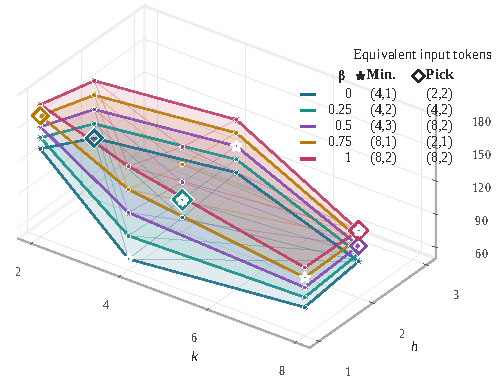
\includegraphics[width=\columnwidth]{fig/experiments/fig09-cache-discount/fig09-cache-discount-sensitivity.pdf}
  \caption{On-cold equivalent cost $C_\beta$ across five cache factors $\beta$. Stars mark empirical minima; diamonds mark planner picks.}
  \label{fig:e4b-beta}
\end{figure}

% The E4c scatter is omitted; its source and experimental records are retained.

\Needspace{327pt}
\subsection{Varying the Limit and Full Ranking}
\label{sec:exp:limit-sweep}
% Cost only: four independently rendered panels in a single-column 2x2 group; quality assets retained.
\begin{figure}[t]
\centering
\setlength{\subfigcapskip}{-1pt}\setlength{\subfigtopskip}{0pt}\setlength{\subfigbottomskip}{0pt}

\includegraphics[width=\columnwidth]{fig/experiments/fig10-limit-sweep/fig10-requested-k-cost-legend.pdf}\par
\vspace{1pt}
\subfigure[\fontsize{6.3bp}{7bp}\selectfont DL20, Off]{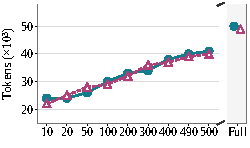
\includegraphics[width=.5\columnwidth]{fig/experiments/fig10-limit-sweep/fig10-requested-k-cost-a-dl20-off.pdf}}%
\subfigure[\fontsize{6.3bp}{7bp}\selectfont DL20, On-cold]{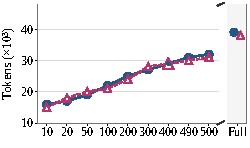
\includegraphics[width=.5\columnwidth]{fig/experiments/fig10-limit-sweep/fig10-requested-k-cost-b-dl20-on-cold.pdf}}\par\vspace{1pt}
\subfigure[\fontsize{6.3bp}{7bp}\selectfont COVID, Off]{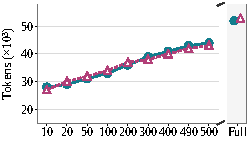
\includegraphics[width=.5\columnwidth]{fig/experiments/fig10-limit-sweep/fig10-requested-k-cost-c-covid-off.pdf}}%
\subfigure[\fontsize{6.3bp}{7bp}\selectfont COVID, On-cold]{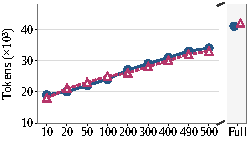
\includegraphics[width=.5\columnwidth]{fig/experiments/fig10-limit-sweep/fig10-requested-k-cost-d-covid-on-cold.pdf}}\par
{\fontsize{6.3bp}{7bp}\selectfont Requested $K$ (categorical); Full is separate}\par
\caption{Equivalent input-token cost across requested \LIMIT~$K$ prefixes and materialized Full ranking under cache Off and On-cold ($\beta{=}0$).}
\label{fig:e5-limit-sweep}
\end{figure}

\endgroup

\section{Related Work}
\label{sec:relatedwork}

\stitle{Semantic query processing.}
LOTUS exposes semantic operators in a dataframe interface and develops execution strategies for operators such as filtering, joins, and top-$K$ ranking~\cite{DBLP:journals/pvldb/PatelJPGAGZ25}.
Unify organizes analytics over unstructured data as pipelines of semantic operators~\cite{DBLP:journals/pvldb/WangLWXL25}.
Other systems use inexpensive proxy models to reduce the number of LLM calls needed to evaluate semantic predicates~\cite{DBLP:journals/pacmmod/ZeighamiSP25,DBLP:journals/corr/abs-2509-12610,DBLP:journals/corr/abs-2601-05536}.
A semantic predicate can be evaluated on one row at a time. Listwise \textsf{ORDER BY} also has to choose which rows to compare together and when to reuse the comparisons.

\stitle{LLM ranking and external merge.}
Pointwise ranking scores items independently~\cite{DBLP:conf/emnlp/DrozdovZD0RWAIM23,DBLP:conf/emnlp/SachanLJAYPZ22}, while pairwise methods aggregate comparisons between items~\cite{DBLP:conf/acl/LuoCH024,DBLP:conf/naacl/QinJHZWYSLLMWB24}.
Listwise ranking orders a batch in one prompt; setwise ranking can select the best item from a batch~\cite{DBLP:conf/sigir/ZhuangZKZ24,DBLP:conf/emnlp/0001YMWRCYR23,DBLP:journals/corr/abs-2305-02156}.
ListK uses listwise tournament and multi-pivot operators for selection and sorting~\cite{DBLP:journals/corr/abs-2603-17223}.
Zhao et al. generate sorted runs and combine them by two-way external merge~\cite{DBLP:journals/corr/abs-2509-00303}.
We retain the run-generation and merge passes of external sorting~\cite{DBLP:journals/csur/Graefe06}. Within each multi-way group, we reuse a ranked window or refresh a single tree path. The planner accounts for which rows are submitted again and how much each group must produce for a given output bound.

\section{Conclusion}
\label{sec:conclusion}
Semantic \textsf{ORDER BY} must assemble a global ranking from listwise calls that can see only part of the input. Our framework organizes these calls as external $k$-way merge. Sliding windows carry uncommitted items between calls, and segmented loser trees replace one segment along the path that next needs input. The same merge groups support full ranking through layer materialization and \LIMIT~$K$ through demand-driven execution. By accounting for both calls and repeated item appearances, the planner can choose the merge family, fan-in, and capacity for the requested output.

\FloatBarrier
\bibliographystyle{ACM-Reference-Format}
\bibliography{ref}
\clearpage
\appendix
\section{Algorithm Correctness}
\label{app:algorithm-proofs}

For Sections~\ref{app:proof-sw}--\ref{app:proof-limit}, fix a strict total order $\prec$ over row identities under instruction $\phi$ with deterministic tie-breaking. A \emph{consistent oracle} returns the restriction of $\prec$ to any batch $B$. Section~\ref{app:proof-inconsistent} requires only that each validated call return a permutation of $B$; distinct input records always retain distinct identities.

\subsection{Sliding-Window Merge}
\label{app:proof-sw}

\begin{lemma}[Safe window prefix]
\label{lem:sw-safe}
For $\prec$-sorted runs and a consistent oracle, each round of Algorithm~\ref{alg:sliding_window_kway_group_merge} emits a nonempty prefix of the $\prec$-sorted union of unemitted rows whenever rows remain, ranking at most $|A|h \le m$ rows (adaptive) or $gh \le kh \le m$ rows (fixed-quota $\mathrm{SW}(k,h)$ on $g \le k$ runs).
\end{lemma}
\begin{proof}
Maintain the invariant that after refill, each active run $u$'s buffered slice $W_u$ is a contiguous prefix of its remaining rows. This holds at $p_u = 0$ and is preserved when removing a prefix per run. If $|A|=1$, the lone run's sorted suffix is appended without a call. Otherwise, for each $u \in A$ with unread items ($p_u + b_u < |R_u|$), let $z_u$ be its last buffered item ($b_u = h \ge 1$) at index $j_u$ in $O$. Emission stops at $t = \min_u j_u$, or drains $O$ if no unread suffix exists.

Every emitted item $x$ precedes or equals $z_u$ in $O$ (hence in $\prec$) for all such $u$. Since unread items of $u$ follow $z_u$ in $\prec$, $x$ precedes all unread suffixes and all survivors $O[t{+}1:]$. Thus the emitted slice is the exact next prefix of the sorted union, and its restriction to each run is a prefix of $W_u$, restoring the invariant. Because $t \ge 1$ (or $|O| \ge 1$), every round makes progress within capacity $m$.
\end{proof}

\subsection{Segmented Loser-Tree Merge}
\label{app:proof-lt}

At internal node $v$, child streams deliver $h$-row blocks (possibly short at exhaustion) into slots $L$ and $R$. Define a slot's \emph{frontier} as its maximum real row under $\prec$ if full ($h$ rows), and $+\infty$ otherwise; retained losers may mix rows from both children.

\begin{lemma}[Node replay and frontier invariant]
\label{lem:lt-node}
Suppose $v$'s slots partition all fetched unforwarded rows, unfetched child rows follow their slot's frontier in $\prec$, and frontier $+\infty$ implies an exhausted child. Algorithm~\ref{alg:replay_segment_node} emits the next block in $\prec$ and restores the invariant once $\mathit{Pointer}(v)$ supplies its next block.
\end{lemma}
\begin{proof}
Initially each slot holds its own child's first block, satisfying the frontier invariant. Let $b_L, b_R$ be the slot frontiers when $L \uplus R$ sorts into $Z$. Any unexhausted child has $h$ slot entries $\preceq$ its frontier, so $Z[1..h]$ is $\preceq \min(b_L, b_R)$ and precedes all unfetched rows; if $|Z| < h$, $b_L = b_R = +\infty$ and emitting $Z$ drains both children.

With virtual $+\infty$ tail padding, the first slot reaching $h$ entries in $Z$ (lines~2--\ref{line:replay-split}) attains $\min(b_L, b_R)$. Meanwhile $\mathit{Loser}(v) = Z[h{+}1..2h]$ retains all unforwarded real rows: if both slots were full, $|\mathit{Loser}(v)| = h$ with maximum $\max(b_L, b_R)$; if either was short, $|\mathit{Loser}(v)| < h$ and the unpointed slot has frontier $+\infty$. Assigning $\mathit{Loser}(v)$ to the unpointed slot preserves frontier $\max(b_L, b_R)$, and refilling from $\mathit{Pointer}(v)$ restores the pointed slot's frontier. For $h{=}2$ with $[1,100]$ and $[3,4]$, replay emits $[1,3]$, retains $[4,100]$ (frontier $100$), and refills the second slot.
\end{proof}

\begin{lemma}[Halving-tree construction and path refresh]
\label{lem:lt-tree}
Algorithms~\ref{alg:loser_tree_kway_group_merge} and~\ref{alg:refresh_loser_tree_path} maintain Lemma~\ref{lem:lt-node} across the halving tree $T$, returning the $\prec$-sorted union within capacity $m$ when $(1+\lceil\log_2 g\rceil)h \le m$.
\end{lemma}
\begin{proof}
View each internal node as a block producer that initializes from its two child blocks and thereafter pulls solely along $\mathit{Pointer}(v)$. Descending from $\textsc{Root}(T)$ traces one path $\mathcal{P}$ ($|\mathcal{P}| \le d = \lceil\log_2 g\rceil$), pulls one leaf block, and replays $\mathcal{P}$ bottom-up while off-path nodes retain valid state. Under a consistent oracle, restricting a packed-init or path-refresh rank map $\rho$ to $L \uplus R$ matches ranking $L \uplus R$ directly, and run-order projection is an identity map; induction on height yields the sorted union (singleton groups pass through without a tree).

Halving $g \ge 2$ leaves gives depth $d = \lceil\log_2 g\rceil$. Since $(d+1)h \le m$ implies $\lfloor m/h \rfloor \ge 2$, each packed initialization cut contracts at least one sibling pair within width $m$, and each refresh ranks at most $(d+1)h \le m$ real rows. At $h{=}1$, $\mathit{Pointer}(v)$ tracks the single winner's source child, recovering the classical loser tree.
\end{proof}

\subsection{Materialization and Demand-Driven Prefix Execution}
\label{app:proof-limit}

\begin{theorem}[Full sortedness and \LIMIT~$K$ equivalence]
\label{thm:full-limit}
Under a consistent oracle, Algorithm~\ref{alg:semantic_external_merge} returns the $\prec$-sorted permutation $\Pi$, and the producer tree (Section~\ref{sec:topk-exec}) returns its first $\min(K,n)$ rows $\Pi_K$.
\end{theorem}
\begin{proof}
Phase~1 sorts disjoint chunks under $\prec$. By Lemmas~\ref{lem:sw-safe} and~\ref{lem:lt-tree} plus singleton pass-through, pass $t$ produces $r_t = \lceil r / k^t \rceil$ disjoint sorted runs, leaving $\Pi$ after $\lceil \log_k r \rceil$ passes ($r \ge 1$). For \LIMIT~$K$, fix initial runs and $\theta$: by induction on tree height, each child's $\textsc{Next}(q)$ delivers the exact next $q$ items of its materialized stream. Every parent refill thus sees identical inputs and state transitions as in Full, buffering unconsumed tails locally and stopping once the root returns $\min(K,n)$ items—even without global consistency whenever corresponding producer calls return matching permutations.
\end{proof}

\subsection{Guarantees under Inconsistent Rank Calls}
\label{app:proof-inconsistent}

\begin{proposition}[Row-identity and run-prefix guarantees]
\label{prop:inconsistent}
If every call returns a batch permutation, both SW and LT($h$) conserve row identities across Full and \LIMIT~$K$. With run-order projection, every LT($h$) output prefix restricts to an exact prefix of each Phase-1 run in original order; unprojected SW need not preserve run prefixes.
\end{proposition}
\begin{proof}
SW removes only emitted identities ($\ge 1$ per round), and LT replay partitions $L \uplus R$ disjointly. If one LT slot is short and one is full, real entries precede $+\infty$ padding, pointing $\mathit{Pointer}(v)$ to the full child so an empty root winner guarantees complete drainage. For any run $R$ in LT, all $R$-rows enter node $v$ via one child contiguously in run order; run-order projection admits only each run's earliest remaining item into $\rho$, so $Z[1..h]$ forwards only the next contiguous prefix of $R$ across all passes and root truncations. In SW with $R_1=(a_1,a_2,a_3,a_4)$, $R_2=(b_1,b_2)$, $h{=}2$, ranking $B$ as $(a_2,b_1,a_1,b_2)$ emits through $a_1$, so \LIMIT~$2$ outputs $(a_2,b_1)$ without $a_1$.
\end{proof}

\section{Additional Cost-Model Analysis}
\label{app:cost-results}

\subsection{Exact Expectation for Single-Item LT Prefixes}
\label{app:cost-exact}

For positive run lengths $\boldsymbol{\ell}$, $h{=}1$, and $1 \le K \le \min_i \ell_i$, packed initialization installs all run heads and emits $\pi_1$ at fixed cost $(A_0, S_0)$. Without prefetching, step $j \in \{2,\dots,K\}$ replaces only $\pi_{j-1}$: since fewer than $K \le \min_i \ell_i$ rows have left each run, source run $i$ has a replacement and full path opponents, incurring deterministic path work $(a_i, s_i)$. Under uniform rank partitioning, rank $j{-}1$ comes from run $i$ with marginal probability $\ell_i / n$; linearity of expectation yields Eq.~\eqref{eq:cost-limit-single} without assuming independent winners. Once $K > \min_i \ell_i$ or $h > 1$, finite replay captures run exhaustion and segment boundaries.

\subsection{Rank-Skew Sensitivity of Sliding-Window Prefixes}
\label{app:cost-skew}

If the top $h$ window ranks fall in one unexhausted run, SW stops at $h$ outputs; balanced interleaving extends the safe prefix. Strong rank clustering can thus cause the uniform model to overestimate safe prefixes on short limits. Because later windows inherit surviving ranks, our simulator retains assigned integer ranks across rounds and passes rather than resampling; more Monte Carlo trials reduce sampling variance under uniform interleaving but do not remove prior mismatch on skewed workloads.

\subsection{First-Row Certification Lower Bound}
\label{app:cost-lowerbound}

Given $r \ge 1$ nonempty $\prec$-sorted runs with no cross-run order and a capacity-$m$ consistent oracle ($m \ge 2$), connect runs in a graph whenever a call ranks items from both. If at least two components remain at termination, shifting one component's ranks above all others preserves all observed permutations while changing $\pi_1$. Since one call touches at most $m$ runs, it merges at most $m - 1$ components, requiring $\lceil (r - 1) / (m - 1) \rceil$ calls—tightly matched by tournament elimination of up to $m$ run heads per call.

\end{document}
